\documentclass[a4paper, 11pt]{article} % Font size (can be 10pt, 11pt or 12pt) and paper size (remove a4paper for US letter paper)

\usepackage[T1]{fontenc}
\usepackage[utf8]{inputenc}
\usepackage[ngerman]{babel}
\usepackage{lmodern}

\usepackage[protrusion=true,expansion=true]{microtype} % Better typography
\usepackage{graphicx} % Required for including pictures
\usepackage{wrapfig} % Allows in-line images
\usepackage{amssymb,amsmath}
\usepackage{subfigure}
\usepackage{cite}
\usepackage{mathpazo} % Use the Palatino font
\linespread{1.05} % Change line spacing here, Palatino benefits from a slight increase by default

\usepackage{tikz-uml}
%\usepackage{tikz}
%\usepackage{ifthen}
%\usepackage{xstring}
%\usepackage{calc}
%\usepackage{pgfopts}

\makeatletter
\renewcommand\@biblabel[1]{\textbf{#1.}} % Change the square brackets for each bibliography item from '[1]' to '1.'
\renewcommand{\@listI}{\itemsep=0pt} % Reduce the space between items in the itemize and enumerate environments and the bibliography

\renewcommand{\maketitle}{ % Customize the title - do not edit title and author name here, see the TITLE block below
\begin{flushright} % Right align
{\LARGE\@title} % Increase the font size of the title

\vspace{50pt} % Some vertical space between the title and author name

{\large\@author} % Author name
\\\@date % Date

\vspace{40pt} % Some vertical space between the author block and abstract
\end{flushright}
}

\title{\textbf{Dokumentation gMix-Simulator GUI}\\ % Title
Benutzer- / Entwicklerhandbuch} % Subtitle

\author{\textsc{Beifuß A. ; Langnickel J. ; Lohmueller J. C. ; Weinschenk M.} % Author
\\{\textit{Universität Hamburg - MIN Falkultaet - Informatik - SVS}}} % Institution

\date{\today} % Date

\begin{document}

\maketitle % Print the title section

%\renewcommand{\abstractname}{Summary} % Uncomment to\texttt{} change the name of the abstract to something else
 
% \begin{abstract}

% \end{abstract}

\tableofcontents

% \hspace*{3,6mm}\textit{Keywords:} lorem , ipsum , dolor , sit amet , lectus % Keywords

\vspace{30pt} % Some vertical space between the abstract and first section

\section{Einleitung} % (fold)
\label{sec:einleitung}

\subsection{gMix} % (fold)
\label{sub:gmix}
Dieser Abschnitt behandelt das Thema Mixe und motiviert die Entwicklung des gMix-Simulators.
% subsection gmix (end)

\subsection{Ziele der GUI} % (fold)ssu
\label{sub:ziele_der_gui}
In diesem Abschnitt werden die unterschiedlichen Benutzergruppen vorgestellt, für die die GUI gedacht ist. Es wird analysiert, welche Anforderungen und Bedürfnisse die jeweiligen Anwendergruppen haben. Entlang der gewonnenen Erkenntnissen soll dann die GUI entwickelt werden, so dass nach Möglichkeit die Anforderungen aller Gruppen zufriedengestellt werden können.
% subsection ziele_der_gui (end)

\subsection{XML vs. Annotations} % (fold)
\label{sub:xml}
In diesem Abschnitt werden wir motivieren, warum wir in der GUI auf Annotations setzen und XML vermeiden.
% subsection xml (end)

% section einleitung (end)

\section{Architektur} % (fold)
\label{sec:architektur}
Die GUI Komponente für den gMix-Simulator basiert gurndlegen auf dem Einsatz von Annotations. Jedes Plug-In, welches für den gMix-Simulator geschrieben wird, muss seine konfigurierbaren Felder über Annotations bekanntmachen. Die GUI ließt bei jedem Start die Plug-Ins aus und erstellt dann dynamisch das Menü, über welches der Benutzer die Plug-Ins konfiguriert. In diesem Abschnitt wird die Architektur der GUI ausführlich dargestellt und das Zusammenspiel der einzelnen Komponenten erklärt.

\subsection{Uebersicht der Architektur} % (fold)
\label{ssub:uebersicht}

\begin{figure}[!htp]
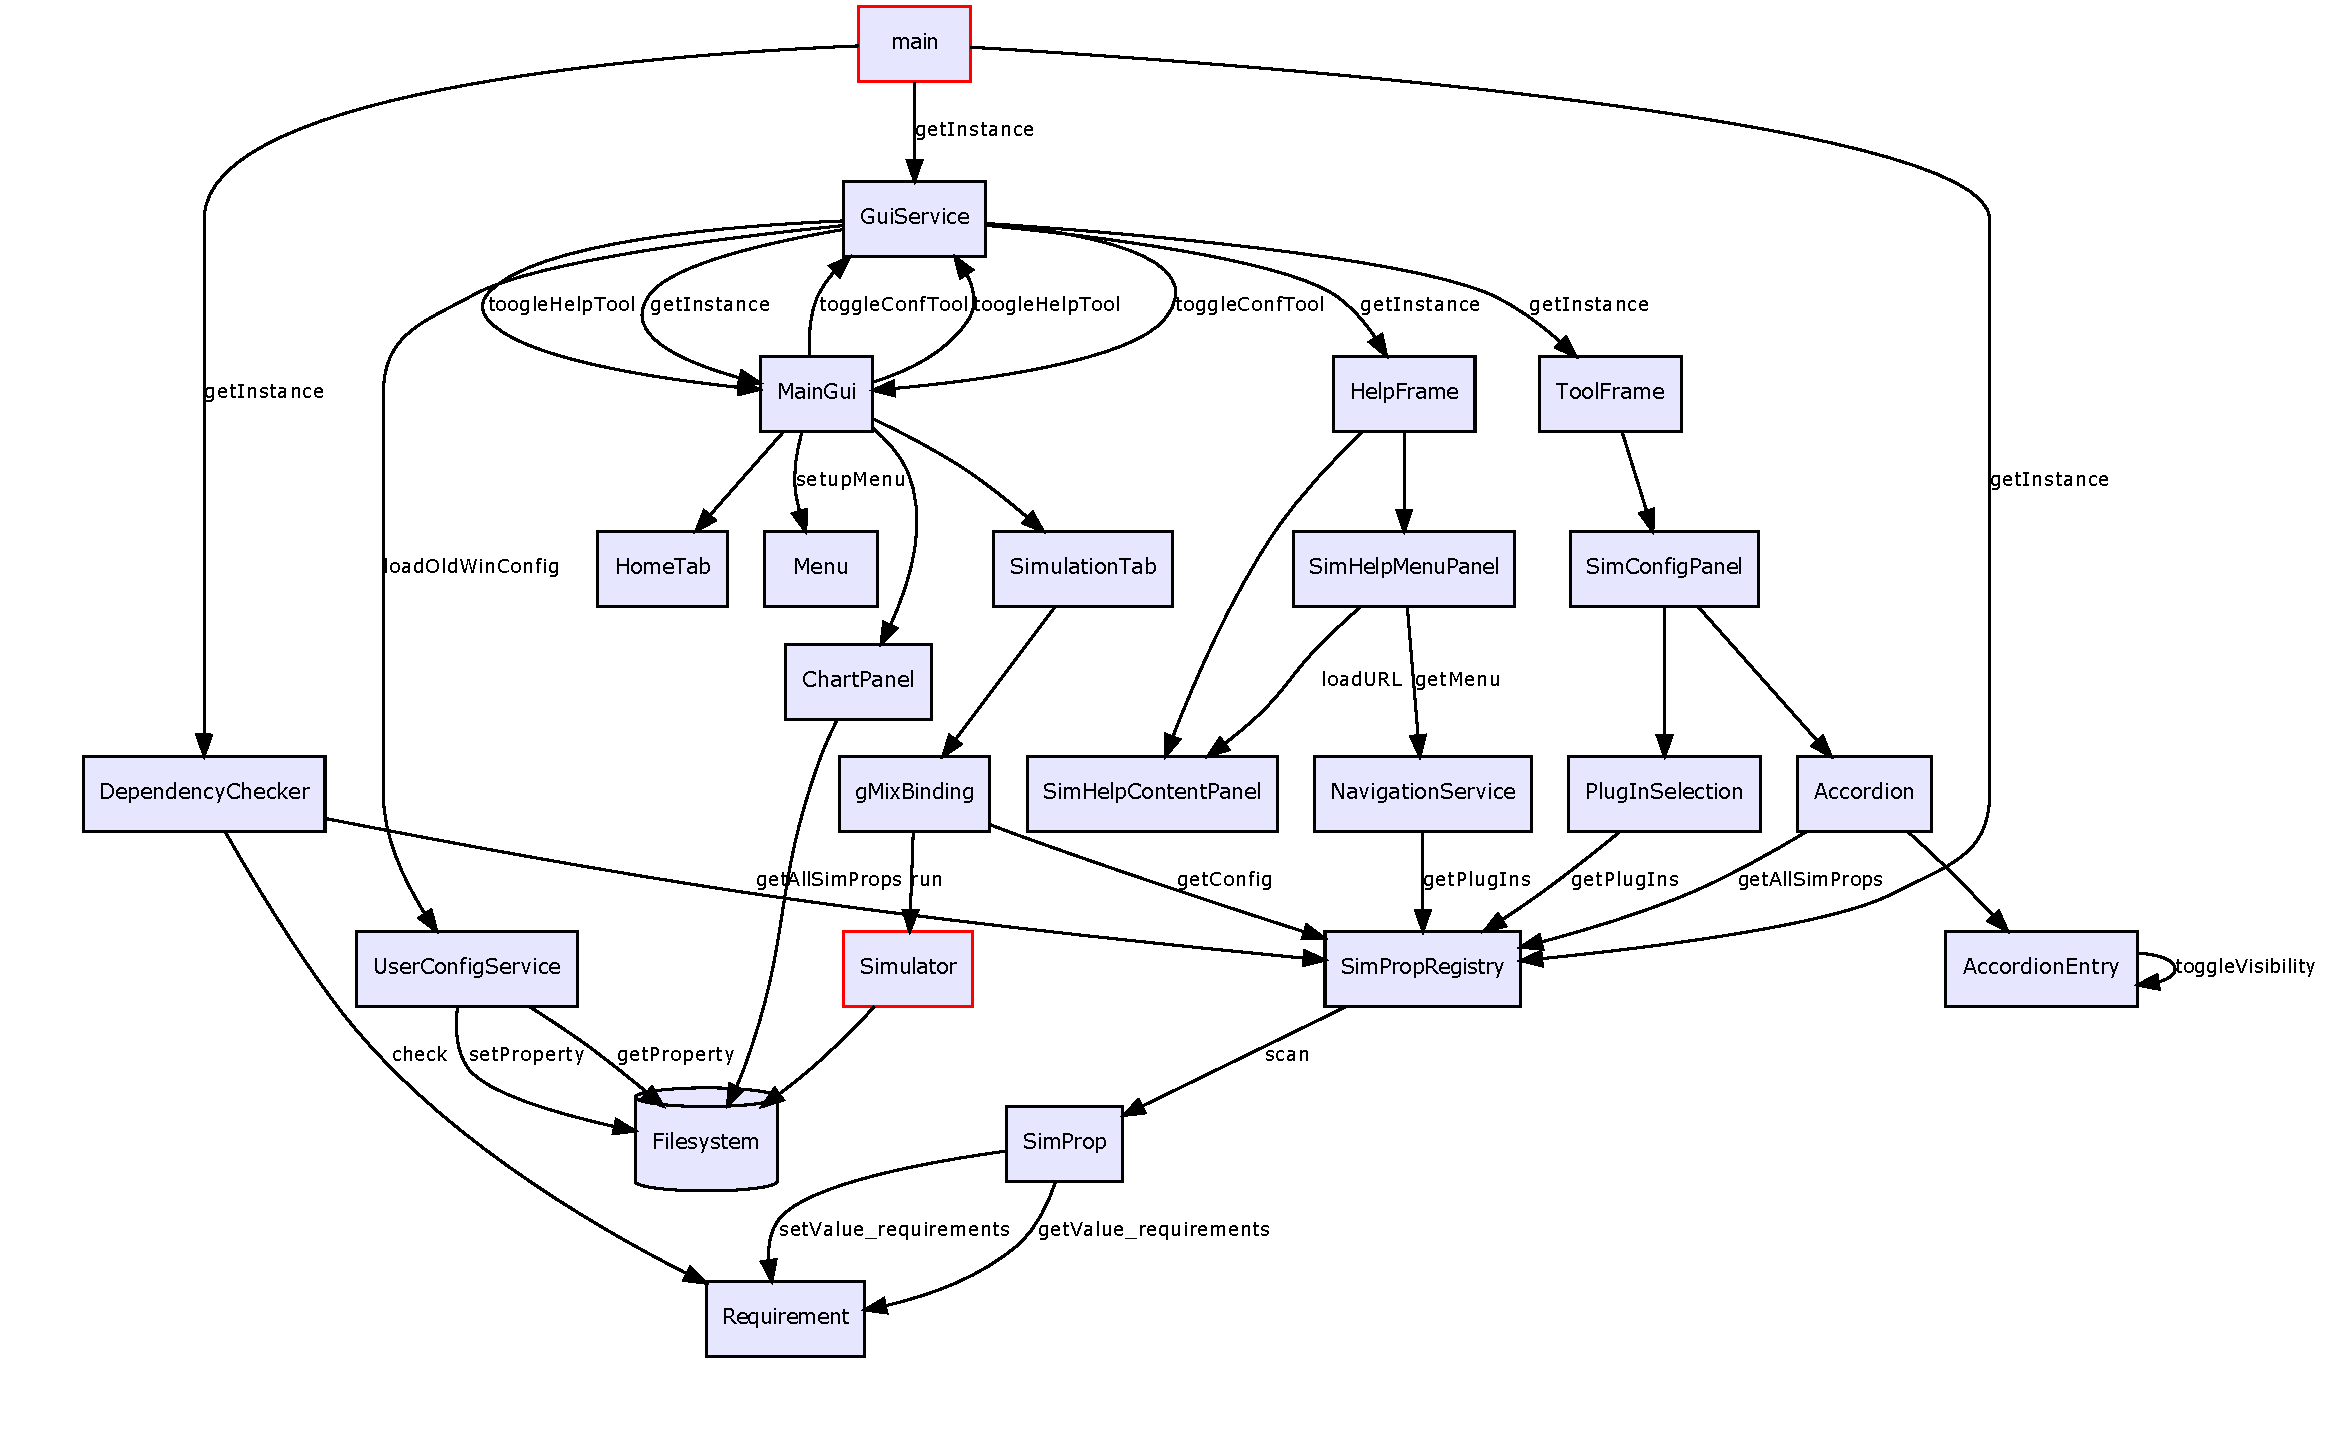
\includegraphics[width=\textwidth]{dot/arch}
\caption{Aufrufhierarchie}
\label{fig:callgraph}
\end{figure}

% subsubsection uebersicht (end)

\subsection{Einzelne Komponenten} % (fold)
\label{ssub:einzelne_komponenten}

\subsubsection{SimPropRegistry}
\label{sssub:simpropregistry}

% subsubsection simpropregistry (end)

\subsubsection{DependencyChecker}
\label{sssub:dependencychecker}

% subsubsection dependencychecker (end)

\subsubsection{GuiService}
\label{sssub:guiservice}

% subsubsection guiservice (end)

% section architektur (end)

\subsection{Feld Annotations} % (fold)
\label{sub:annotations}
Dieser Abschnitt beschreibt die unterschiedlichen Annotation-Typen, welche unsere GUI bereistellt.
% subsection annotations (end)

\subsubsection{Feld Annotations} % (fold)
\label{ssub:feld_annotations}

\begin{figure}[!htp]
\begin{tikzpicture}
\umlsimpleclass[fill=blue!10]{SimProp}
\umlemptyclass[x=-4.5, y=-2, fill=blue!10]{BoolProp}
\umlemptyclass[x=-1.5, y=-2, fill=blue!10]{IntProp}
\umlemptyclass[x=1.5, y=-2, fill=blue!10]{FloatProp}
\umlemptyclass[x=4.5, y=-2, fill=blue!10]{StringProp}
\umlVHVinherit[arm2=-1.2cm]{BoolProp}{SimProp}
\umlVHVinherit[arm2=-1.2cm]{IntProp}{SimProp}
\umlVHVinherit[arm2=-1.2cm]{FloatProp}{SimProp}
\umlVHVinherit[arm2=-1.2cm]{StringProp}{SimProp}
\end{tikzpicture}
\caption{Vererbung der Feld Annotations}
\label{fig:field_annotations}
\end{figure}

% subsubsection feld_annotations (end)

\subsubsection{Plug-In Annotations} % (fold)
\label{ssub:subsection_name}
Neben den Feld Annotations gibt es eine weitere Klasse von Annotations, die Plug-In Annotations. 
% subsection subsection_name (end)

\section{Features} % (fold)
\label{sec:features}
Hier sollen später die Features unserer GUI aufgelistet und erklärt werden!

TEST \cite{dummy:svs}.
% section features (end)

\bibliographystyle{plain}

\bibliography{references}

%----------------------------------------------------------------------------------------

\end{document}